\documentclass{article}
\usepackage[utf8]{inputenc}
\usepackage{amsmath}
\usepackage{graphicx}
\graphicspath{ {./images/} }

\title{TDT4117 - Assignment 4}
\author{Marius Aarsnes}
\date{November 2018}

\begin{document}

\maketitle

\section{Task 1: Page rank and HITS}

\subsection{Compare page rank and HITS and briefly describe the main ideas of both approaches and point out their differences.}

HITS was developed by Jon Kleinberg. The algorithm makes use of the link structure of the web in order to discover and rank pages relevant for a particular topic. Instead of simply looking at the occurrences of relevant words to the query, the method tries to implement some "logic" by looking at related topics or pages. The main advantage to HITS is its ability to rank pages according to the query topic. Some of the disadvantages with HITS are that the neighbourhood graph must be built on the fly therefore minor changes to the web could significantly change the authority and hub scores. Also, topic-drift is another problem where the neighbourhood graph could contain nodes which have high authority scores for unrelated topics to the original query. 

\vspace{2mm}

\noindent PageRank was developed by Google. PageRank is similar to HITS, however, PageRank does not take into account the user's query. The main idea behind PageRank is that a page is important if it is pointed to by other important pages. The PageRank of a page is determined by the summing the PageRanks of all the pages that point to yours. Advantages to PageRank is that the algorithm is robust against Spam, since it is difficult to add in-links to their page from other important pages. Also, PageRank is a global measure and is query independent. A disadvantage of PageRank are that it favors older pages, since new pages will not have many links unless it is a part of an existing site. 

\newpage
\subsection{Given the $G=\{V,E\}$ given in the assignment, compute hub and authority scores for webpages labeled as A, B, C and D using HITS algorithm. Perform at least 3 iterations of the algorithm and illustrate your computations by providing formulas filled with values for at least one iteration.}

To solve the assignment, the following expressions and assumptions have been used:

\begin{flalign}
    a_i^{(k)} & = \sum_j h_j^{(k-1)}, \text{ where} \; e_{ij} \in E\\
    \vec{a}^{(k)} &=L^T\vec{h}^{(k-1)} \; \text{ and } \; \vec{h}^{(k)} =L\vec{a}^{(k)} \\
    L_{ij} &= 
    \begin{cases}
    1 & \text{if there exists $i$ and $j$ such that $ e_{ij} \in E$}; \\
    0 & \text{otherwise.}
    \end{cases} \\
    L_{ij} &= 
    \begin{bmatrix}
         0 & 1 & 1 & 1 \\
         1 & 0 & 1 & 0 \\
         0 & 0 & 0 & 1 \\
         0 & 0 & 0 & 0
    \end{bmatrix} \\
    L^T & =
    \begin{bmatrix}
        0 & 1 & 0 & 0 \\
        1 & 0 & 0 & 0 \\
        1 & 1 & 0 & 0 \\
        1 & 0 & 1 & 0 \\
    \end{bmatrix} \\
        \vec{h}^{0} &= 
    \begin{bmatrix}
        1 \\
        1 \\
        1 \\
        1
    \end{bmatrix}
\end{flalign}

\noindent Where $\vec{a}^{(k)}$ and $\vec{h}^{(k)}$ are vectors comprising the authority and hub scores for each of the n nodes in the graph.

\vspace{2mm}

Iteration 1: 
\vspace{2mm}
\begin{flalign*}
    \vec{a}^1  &= L^T\vec{h}^0 = 
        \begin{bmatrix} 
            0 & 1 & 0 & 0 \\
            1 & 0 & 0 & 0 \\
            1 & 1 & 0 & 0 \\
            1 & 0 & 1 & 0 
        \end{bmatrix} \times 
        \begin{bmatrix}
            1 \\
            1 \\
            1 \\
            1 
        \end{bmatrix} =
        \begin{bmatrix}
            1 \\
            1 \\
            2 \\
            2 \\
        \end{bmatrix} \\
    \vec{h}^1 & = L\vec{a}^1 \;\;= 
    \begin{bmatrix}
         0 & 1 & 1 & 1 \\
         1 & 0 & 1 & 0 \\
         0 & 0 & 0 & 1 \\
         0 & 0 & 0 & 0
    \end{bmatrix} \times 
    \begin{bmatrix}
            1 \\
            1 \\
            2 \\
            2 \\
    \end{bmatrix} = 
    \begin{bmatrix}
        5 \\
        3 \\
        2 \\
        0 
    \end{bmatrix}
\end{flalign*}

\vspace{2mm}

Now we normalise the values and get:

\begin{flalign*}
    \vec{a}^1 & = \frac{\vec{a}^1}{\sqrt{\sum_j \vec{a_j}^1}} = 
    \begin{bmatrix}
        0.316 \\
        0.316 \\
        0.632 \\
        0.632
    \end{bmatrix} \\
    \vec{h}^1 &= \frac{\vec{h}^1}{\sqrt{\sum_j \vec{h_j}^1}} = 
    \begin{bmatrix}
        0.811 \\
        0.487 \\
        0.324 \\
        0
    \end{bmatrix}
\end{flalign*}

\vspace{2mm}

Iteration 2:

\begin{flalign*}
    \vec{a}^2  &= L^T\vec{h}^1 = 
        \begin{bmatrix} 
            0 & 1 & 0 & 0 \\
            1 & 0 & 0 & 0 \\
            1 & 1 & 0 & 0 \\
            1 & 0 & 1 & 0 
        \end{bmatrix} \times 
        \begin{bmatrix}
            0.811 \\
            0.487 \\
            0.324 \\
            0
        \end{bmatrix} = 
        \begin{bmatrix}
            0.487 \\
            0.811 \\
            1.298 \\
            1.135
        \end{bmatrix} \\
    \vec{h}^2  & = L\vec{a}^2 \; \;= 
        \begin{bmatrix}
            0 & 1 & 1 & 1 \\
            1 & 0 & 1 & 0 \\
            0 & 0 & 0 & 1 \\
            0 & 0 & 0 & 0
        \end{bmatrix} \times 
        \begin{bmatrix}
            0.487 \\
            0.811 \\
            1.298 \\
            1.135
        \end{bmatrix} =
        \begin{bmatrix}
            4.244 \\
            1.785 \\
            1.135 \\
            0
        \end{bmatrix}
\end{flalign*}

\vspace{2mm}

Now we normalise the values and get:

\begin{flalign*}
    \vec{a}^2 & = \frac{\vec{a}^2}{\sqrt{\sum_j \vec{a_j}^2}} = 
    \begin{bmatrix}
        0.248 \\
        0.412 \\
        0.660 \\
        0.577
    \end{bmatrix} \\
    \vec{h}^2 &= \frac{\vec{h}^2}{\sqrt{\sum_j \vec{h_j}^2}} = 
    \begin{bmatrix}
        0.895 \\
        0.376 \\
        0.239 \\
        0
    \end{bmatrix}
\end{flalign*}

Iteration 3:

\vspace{2mm}

\begin{flalign*}
    \vec{a}^3  &= L^T\vec{h}^2 = 
        \begin{bmatrix} 
            0 & 1 & 0 & 0 \\
            1 & 0 & 0 & 0 \\
            1 & 1 & 0 & 0 \\
            1 & 0 & 1 & 0 
        \end{bmatrix} \times 
        \begin{bmatrix}
            0.895 \\
            0.376 \\
            0.239 \\
            0
        \end{bmatrix} =
        \begin{bmatrix}
            0.376 \\
            0.895 \\
            1.271 \\
            1.134
        \end{bmatrix}\\
    \vec{h}^3  & = L\vec{a}^3 \; \;= 
        \begin{bmatrix}
            0 & 1 & 1 & 1 \\
            1 & 0 & 1 & 0 \\
            0 & 0 & 0 & 1 \\
            0 & 0 & 0 & 0
        \end{bmatrix} \times 
        \begin{bmatrix}
            0.376 \\
            0.895 \\
            1.271 \\
            1.134
        \end{bmatrix} =
        \begin{bmatrix}
            3.3 \\
            1.647 \\
            1.134 \\
            0
        \end{bmatrix}
\end{flalign*}

\vspace{2mm}

Now we normalise the values and get:

\vspace{2mm}

\begin{flalign*}
    \vec{a}^3 & = \frac{\vec{a}^3}{\sqrt{\sum_j \vec{a_j}^3}} = 
    \begin{bmatrix}
        0.192 \\
        0.457 \\
        0.650 \\
        0.578
    \end{bmatrix} \\
    \vec{h}^3 &= \frac{\vec{h}^3}{\sqrt{\sum_j \vec{h_j}^3}} = 
    \begin{bmatrix}
        0.855 \\
        0.427 \\
        0.294 \\
        0
    \end{bmatrix}
\end{flalign*}
\section{Task 2 : Structured Indexing and Retrieval in Lucene}
\subsection{Subtask A}
I got a little confused by the assignment as there were, in my eyes, some inconsistencies in the text. First it says that ID should be one of the fields that the documents should be indexed by. Later in the text ID is not mentioned as one of the fields that should be searchable. Also, in the handed-out code the comments says to add 'path' as one of the indexed fields. In the end i have decided to add ID, and not path as on of the searchable fields. I realise this does not make much sense seeing as all the ID's are integers.

\subsection{Subtask B}
Luke is a program which uses the indexes we generated using Lucene, in the previous task to show and modify content in different ways. By making sure that Lucene indexed the fields we wanted to sort by/search in, we generated index-files which we later used in Luke. This way we could search for given terms in the different fields in the documents. In this specific case we searched for "Vancouver".

The results can be viewed in the images below. Due to some scaling issues, the images can also be found in a separate folder "images".
\begin{figure}[h]

    \centering
    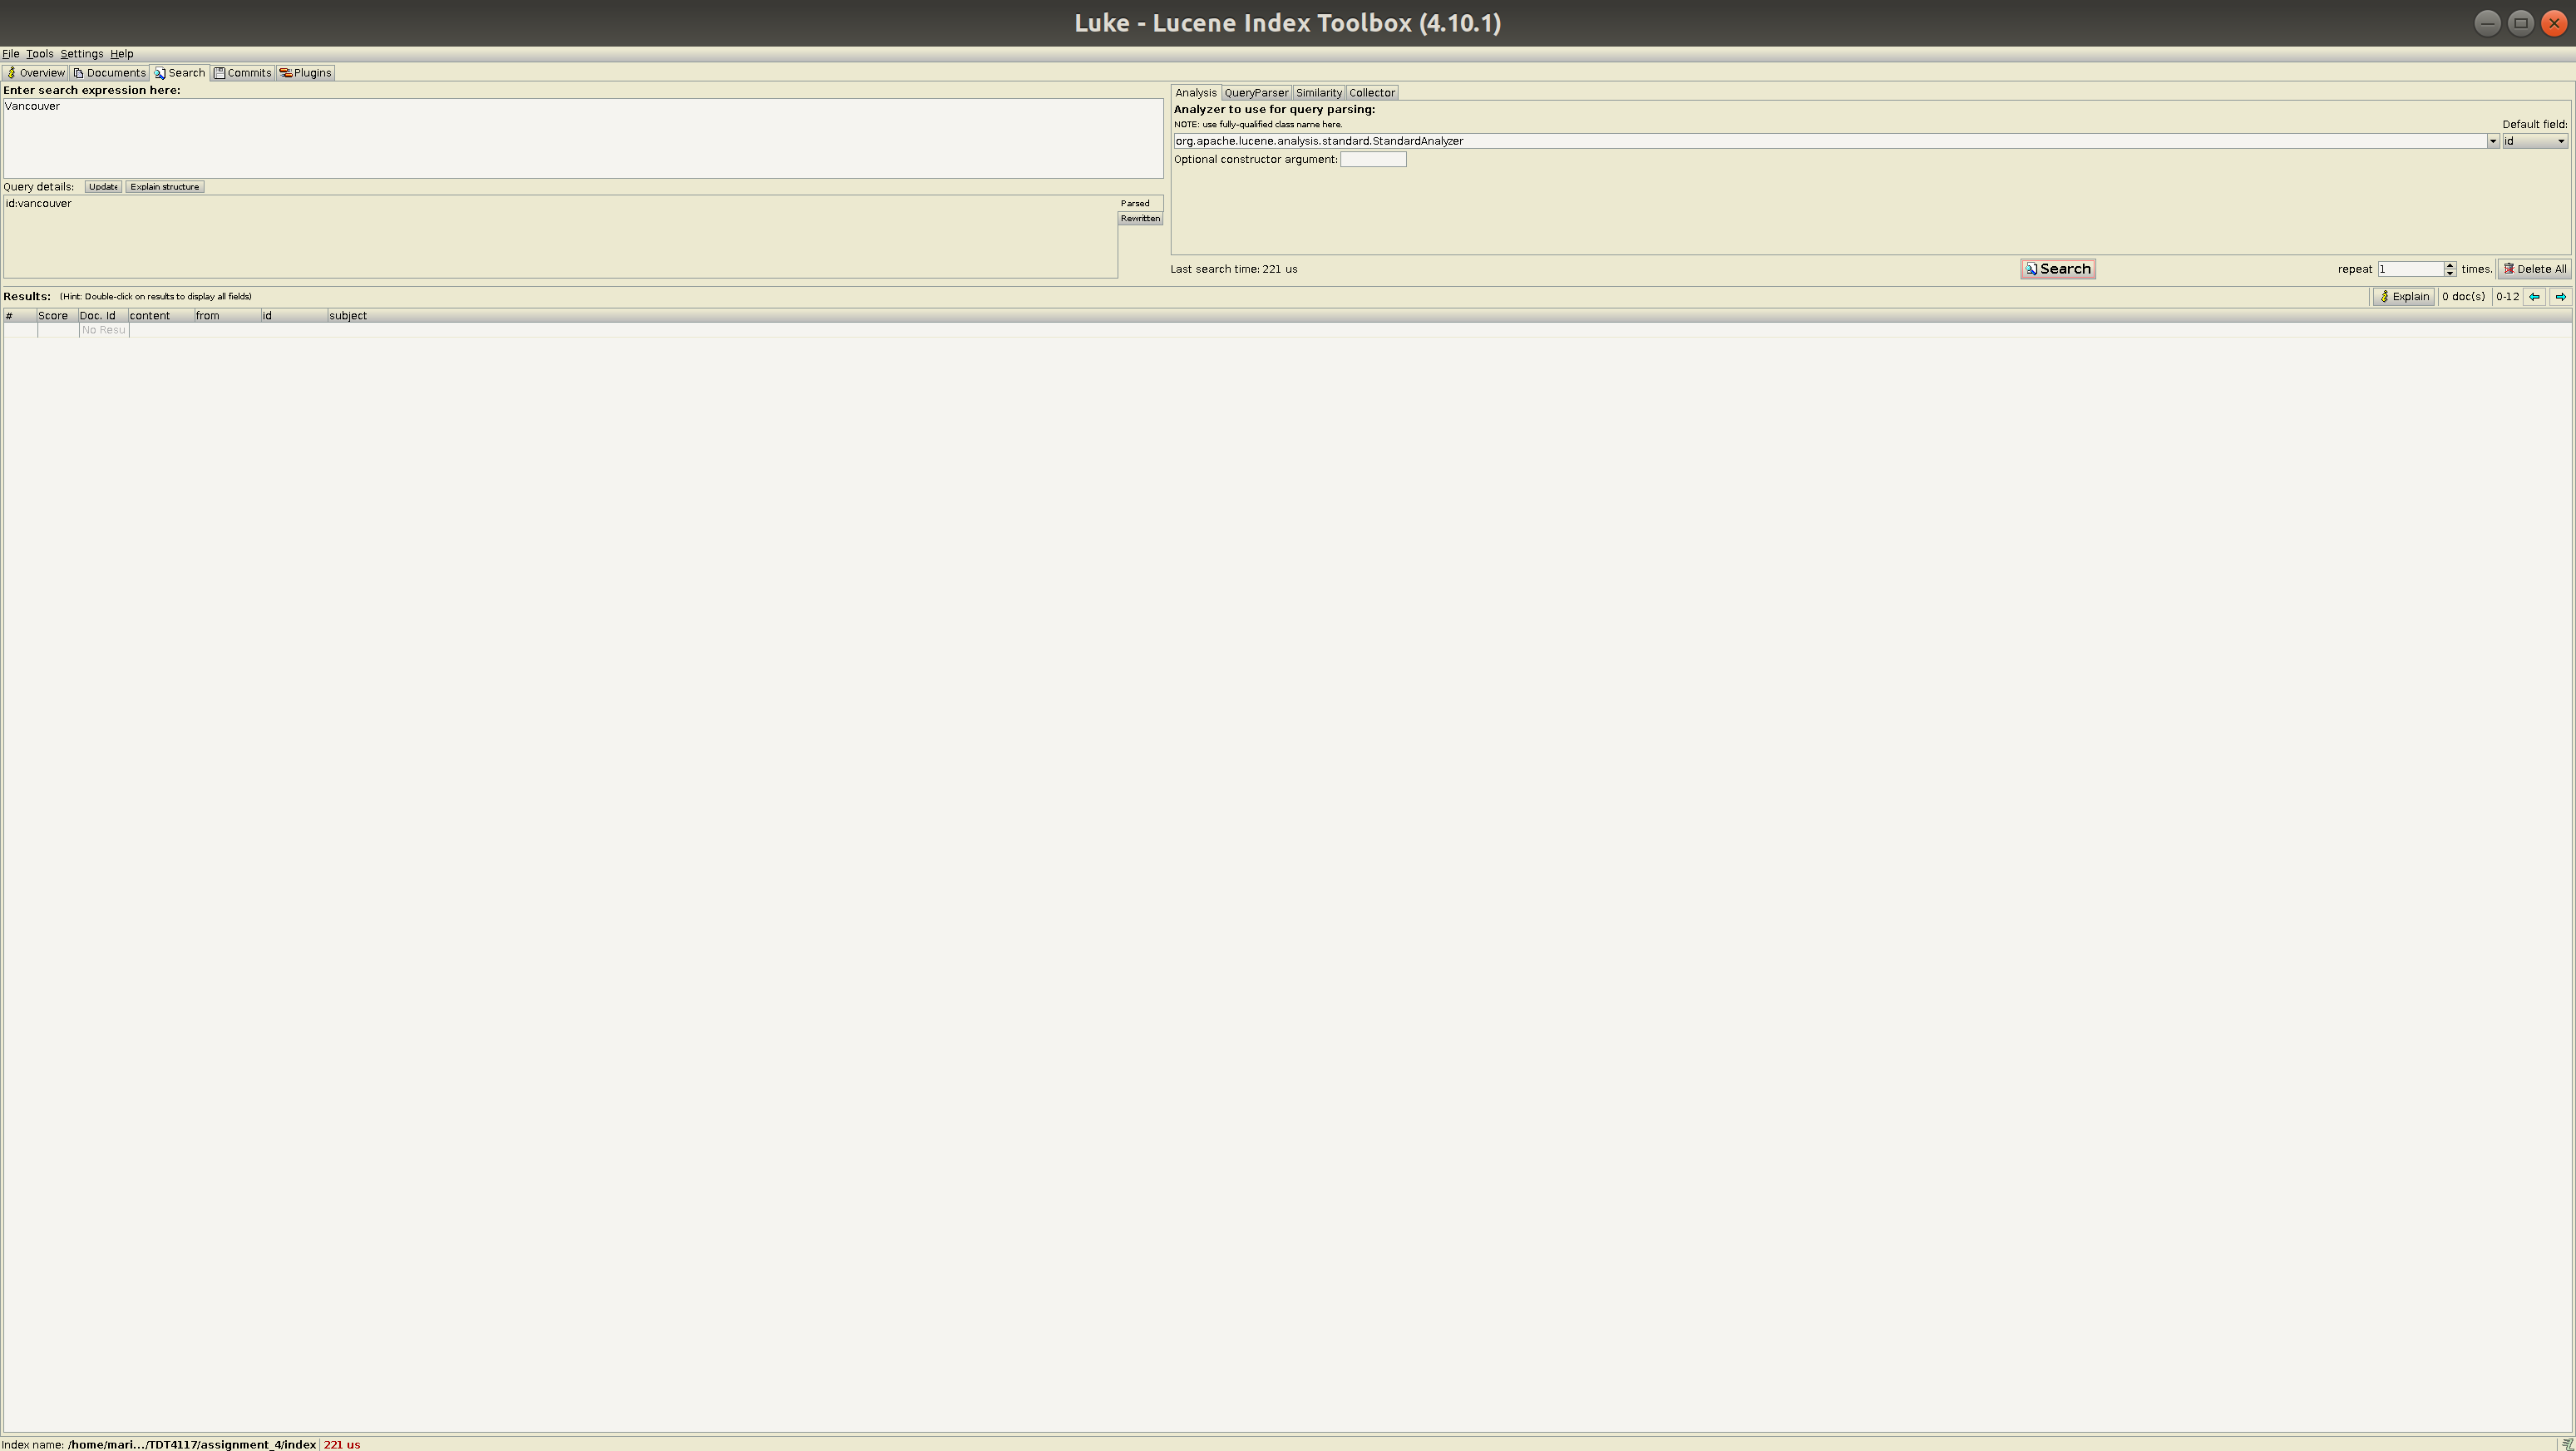
\includegraphics[width=\textwidth]{id}
    \caption{Searched for Vancouver in id}
    \label{fig:id}
\end{figure}

\begin{figure}[h]
    \centering
    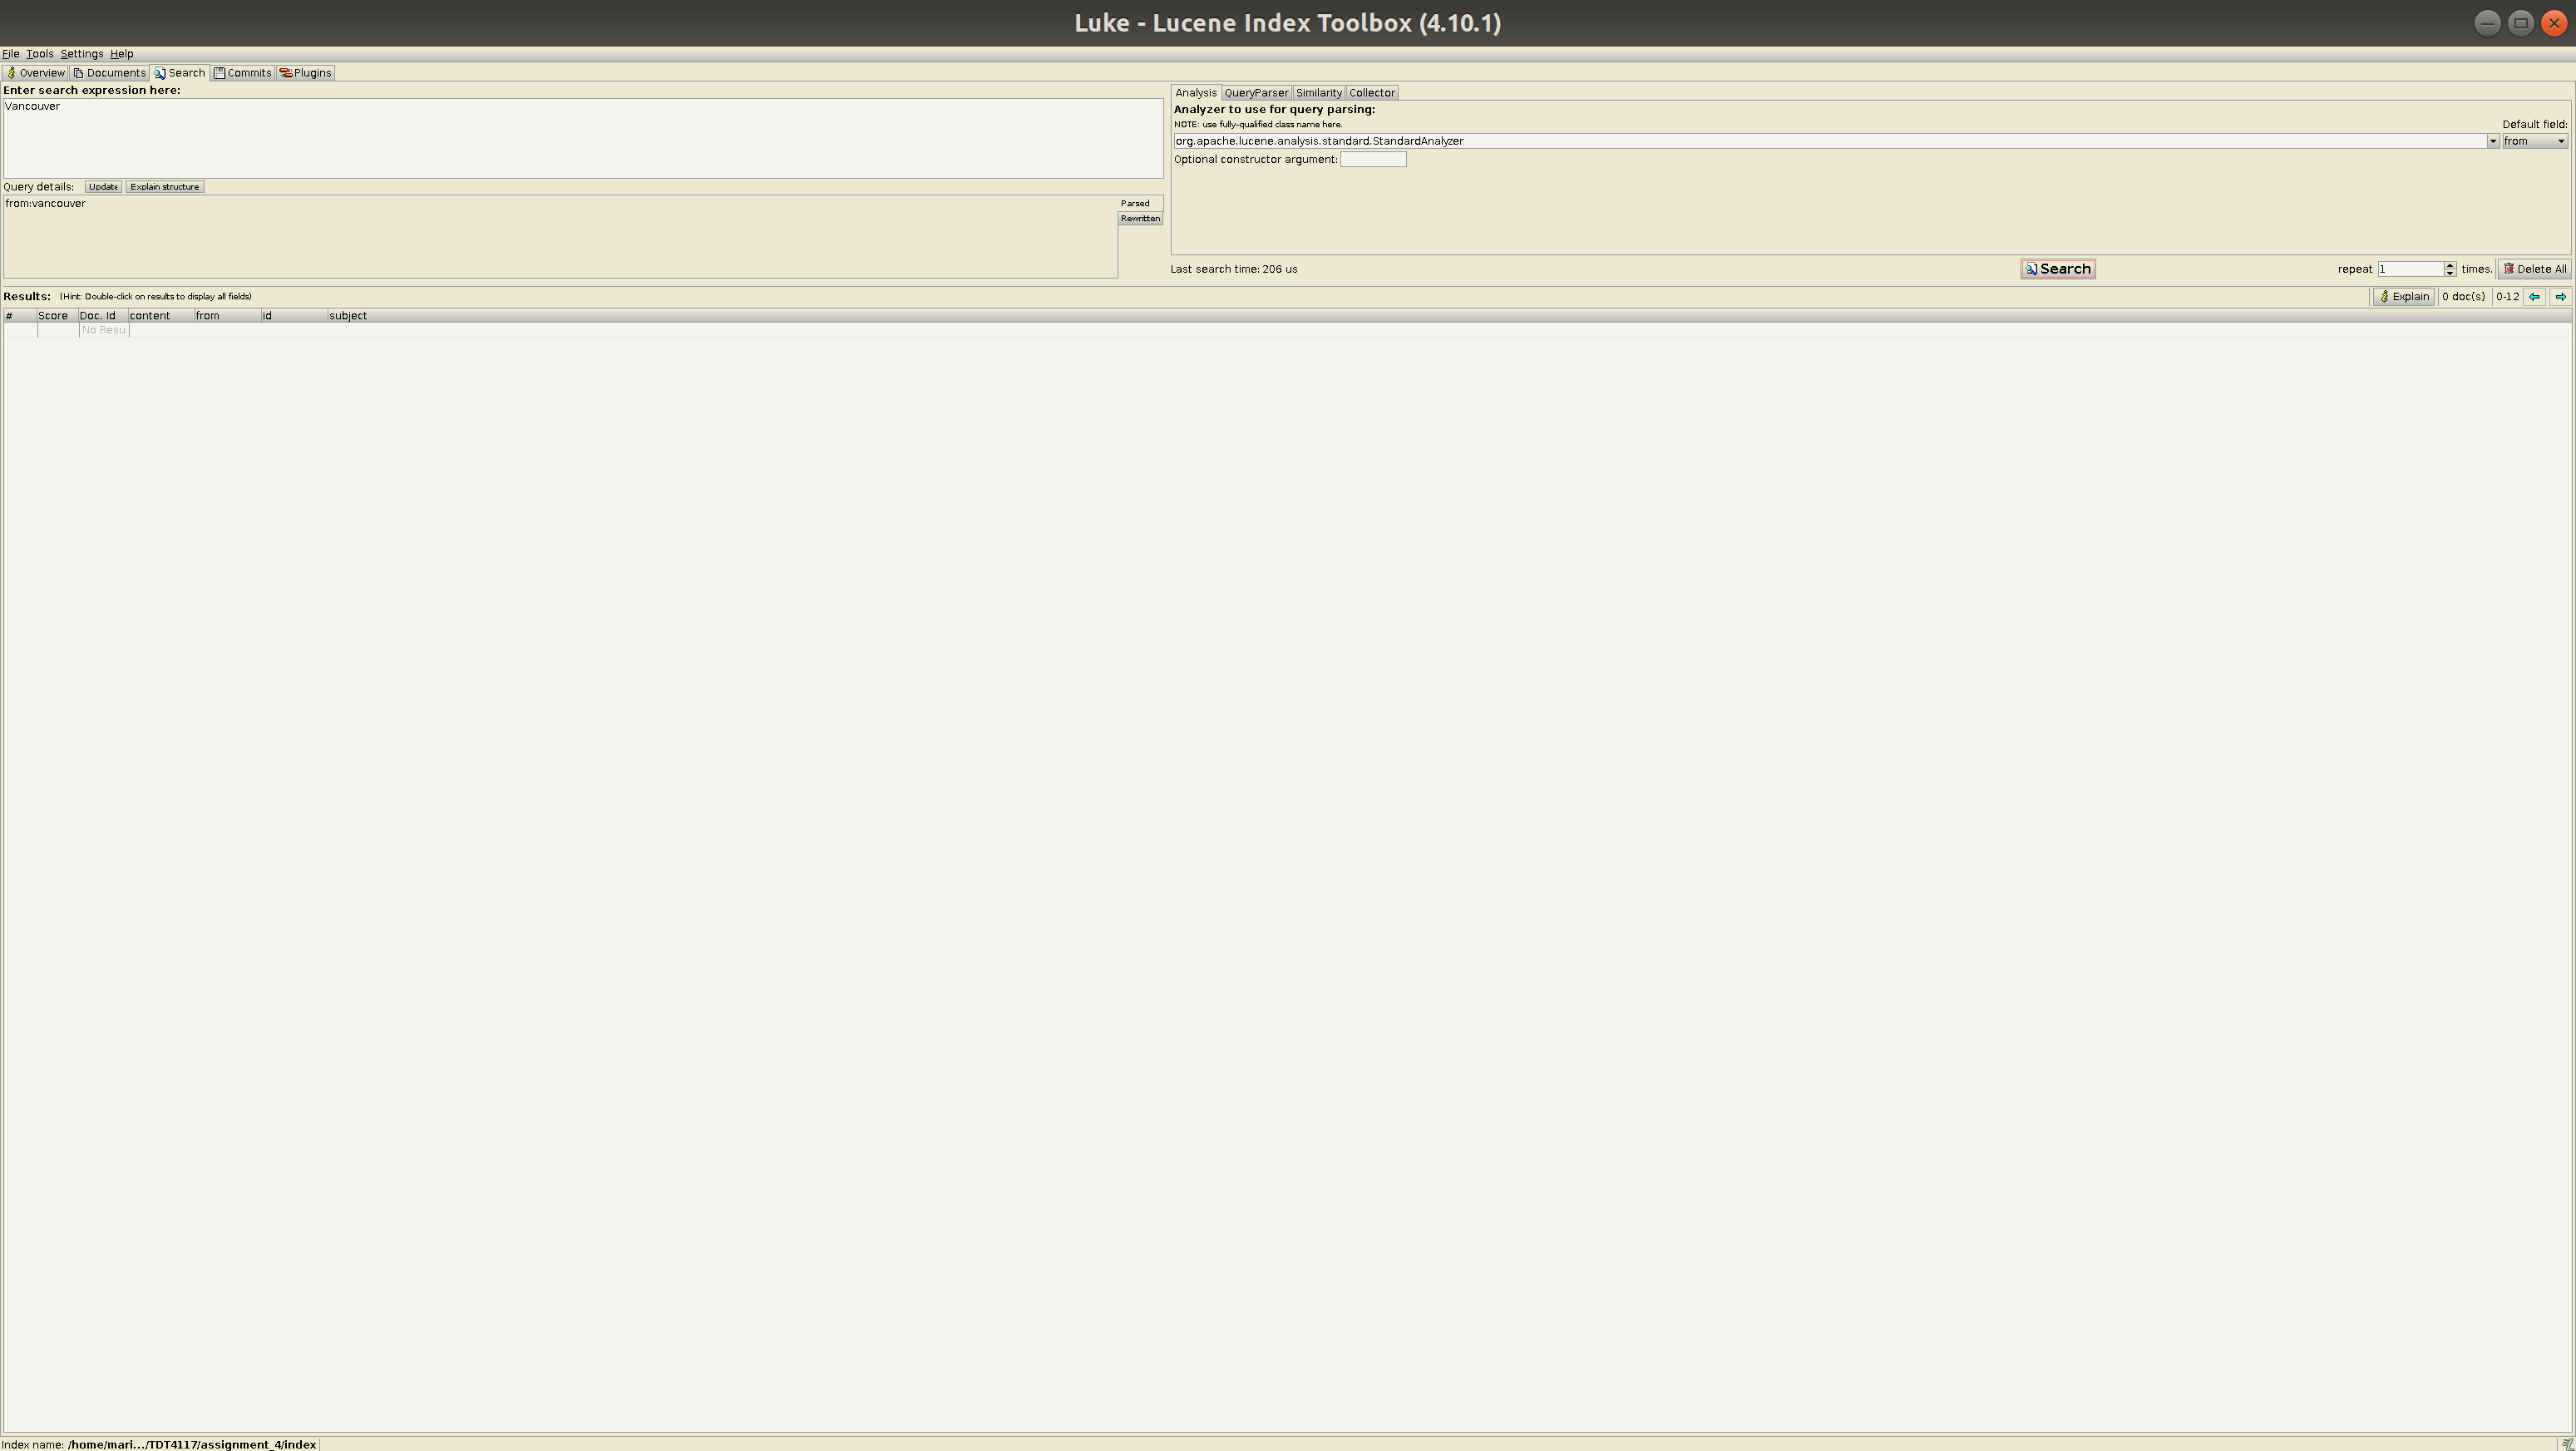
\includegraphics[width=\textwidth]{from}
    \caption{Searched for Vancouver in from}
    \label{fig:from}
\end{figure}

\begin{figure}[h]
    \centering
    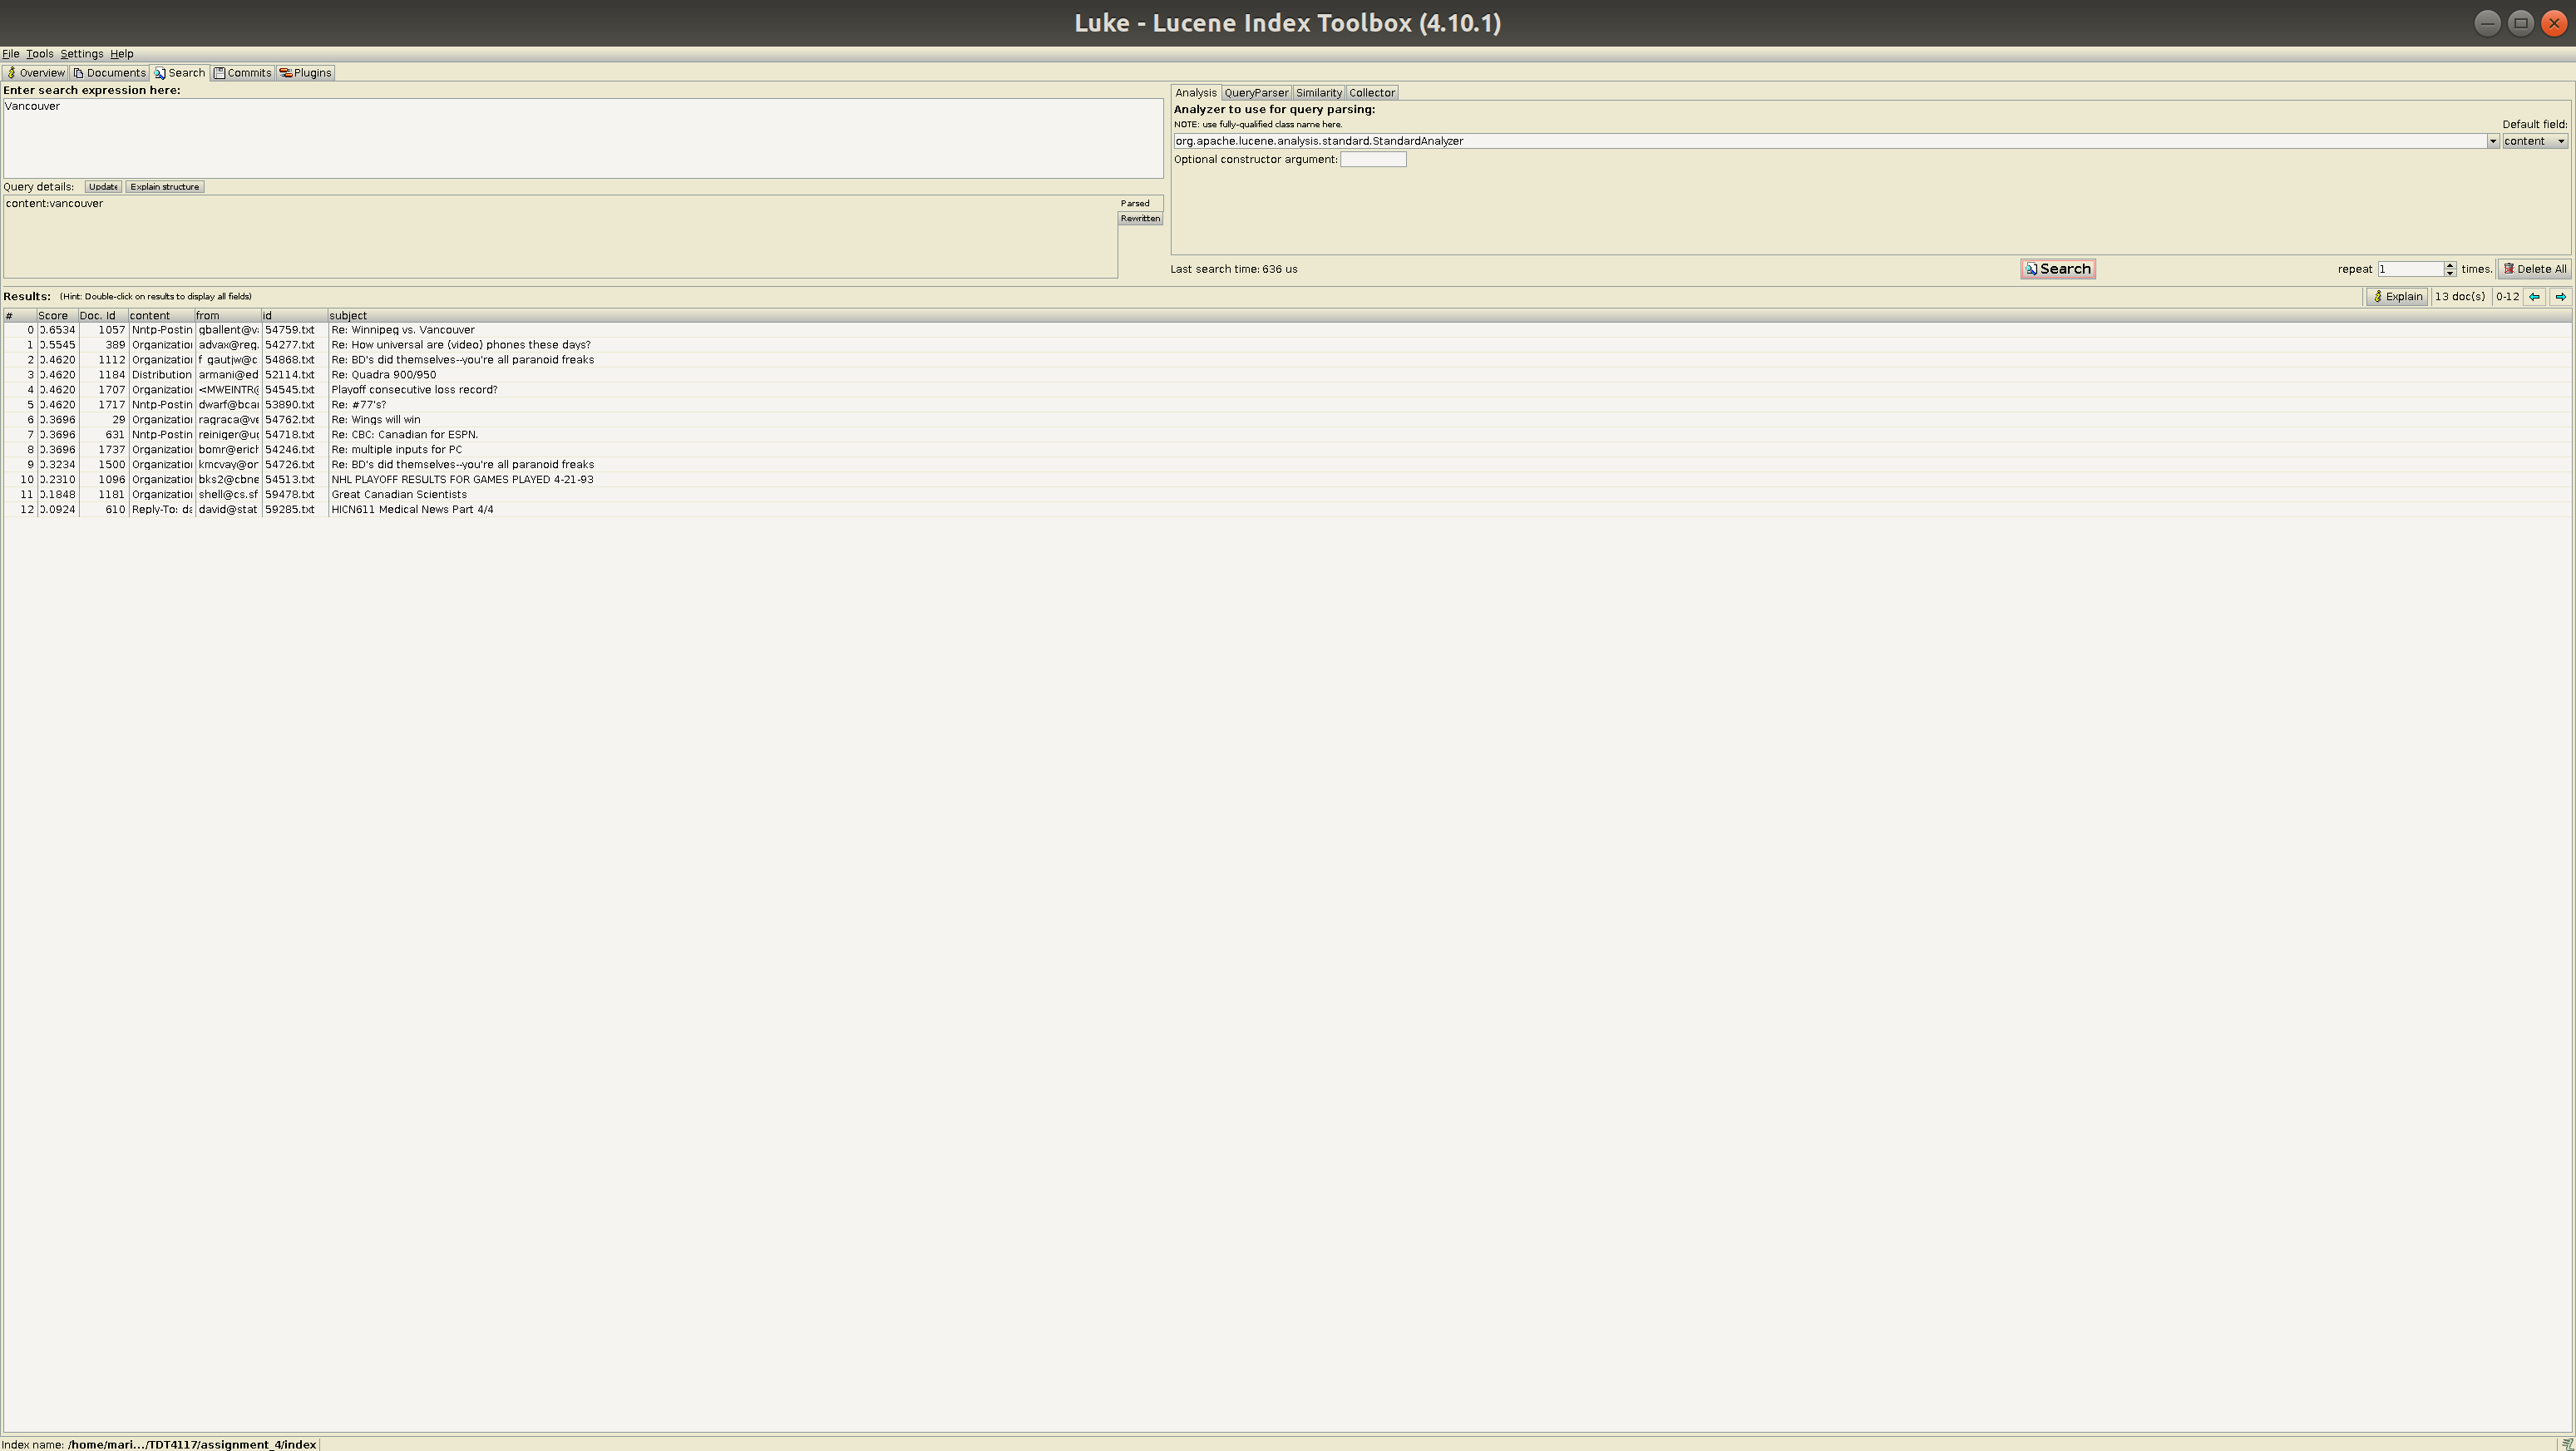
\includegraphics[width=\textwidth]{content}
    \caption{Searched for Vancouver in content}
    \label{fig:content}
\end{figure}

\begin{figure}[h]
    \centering
    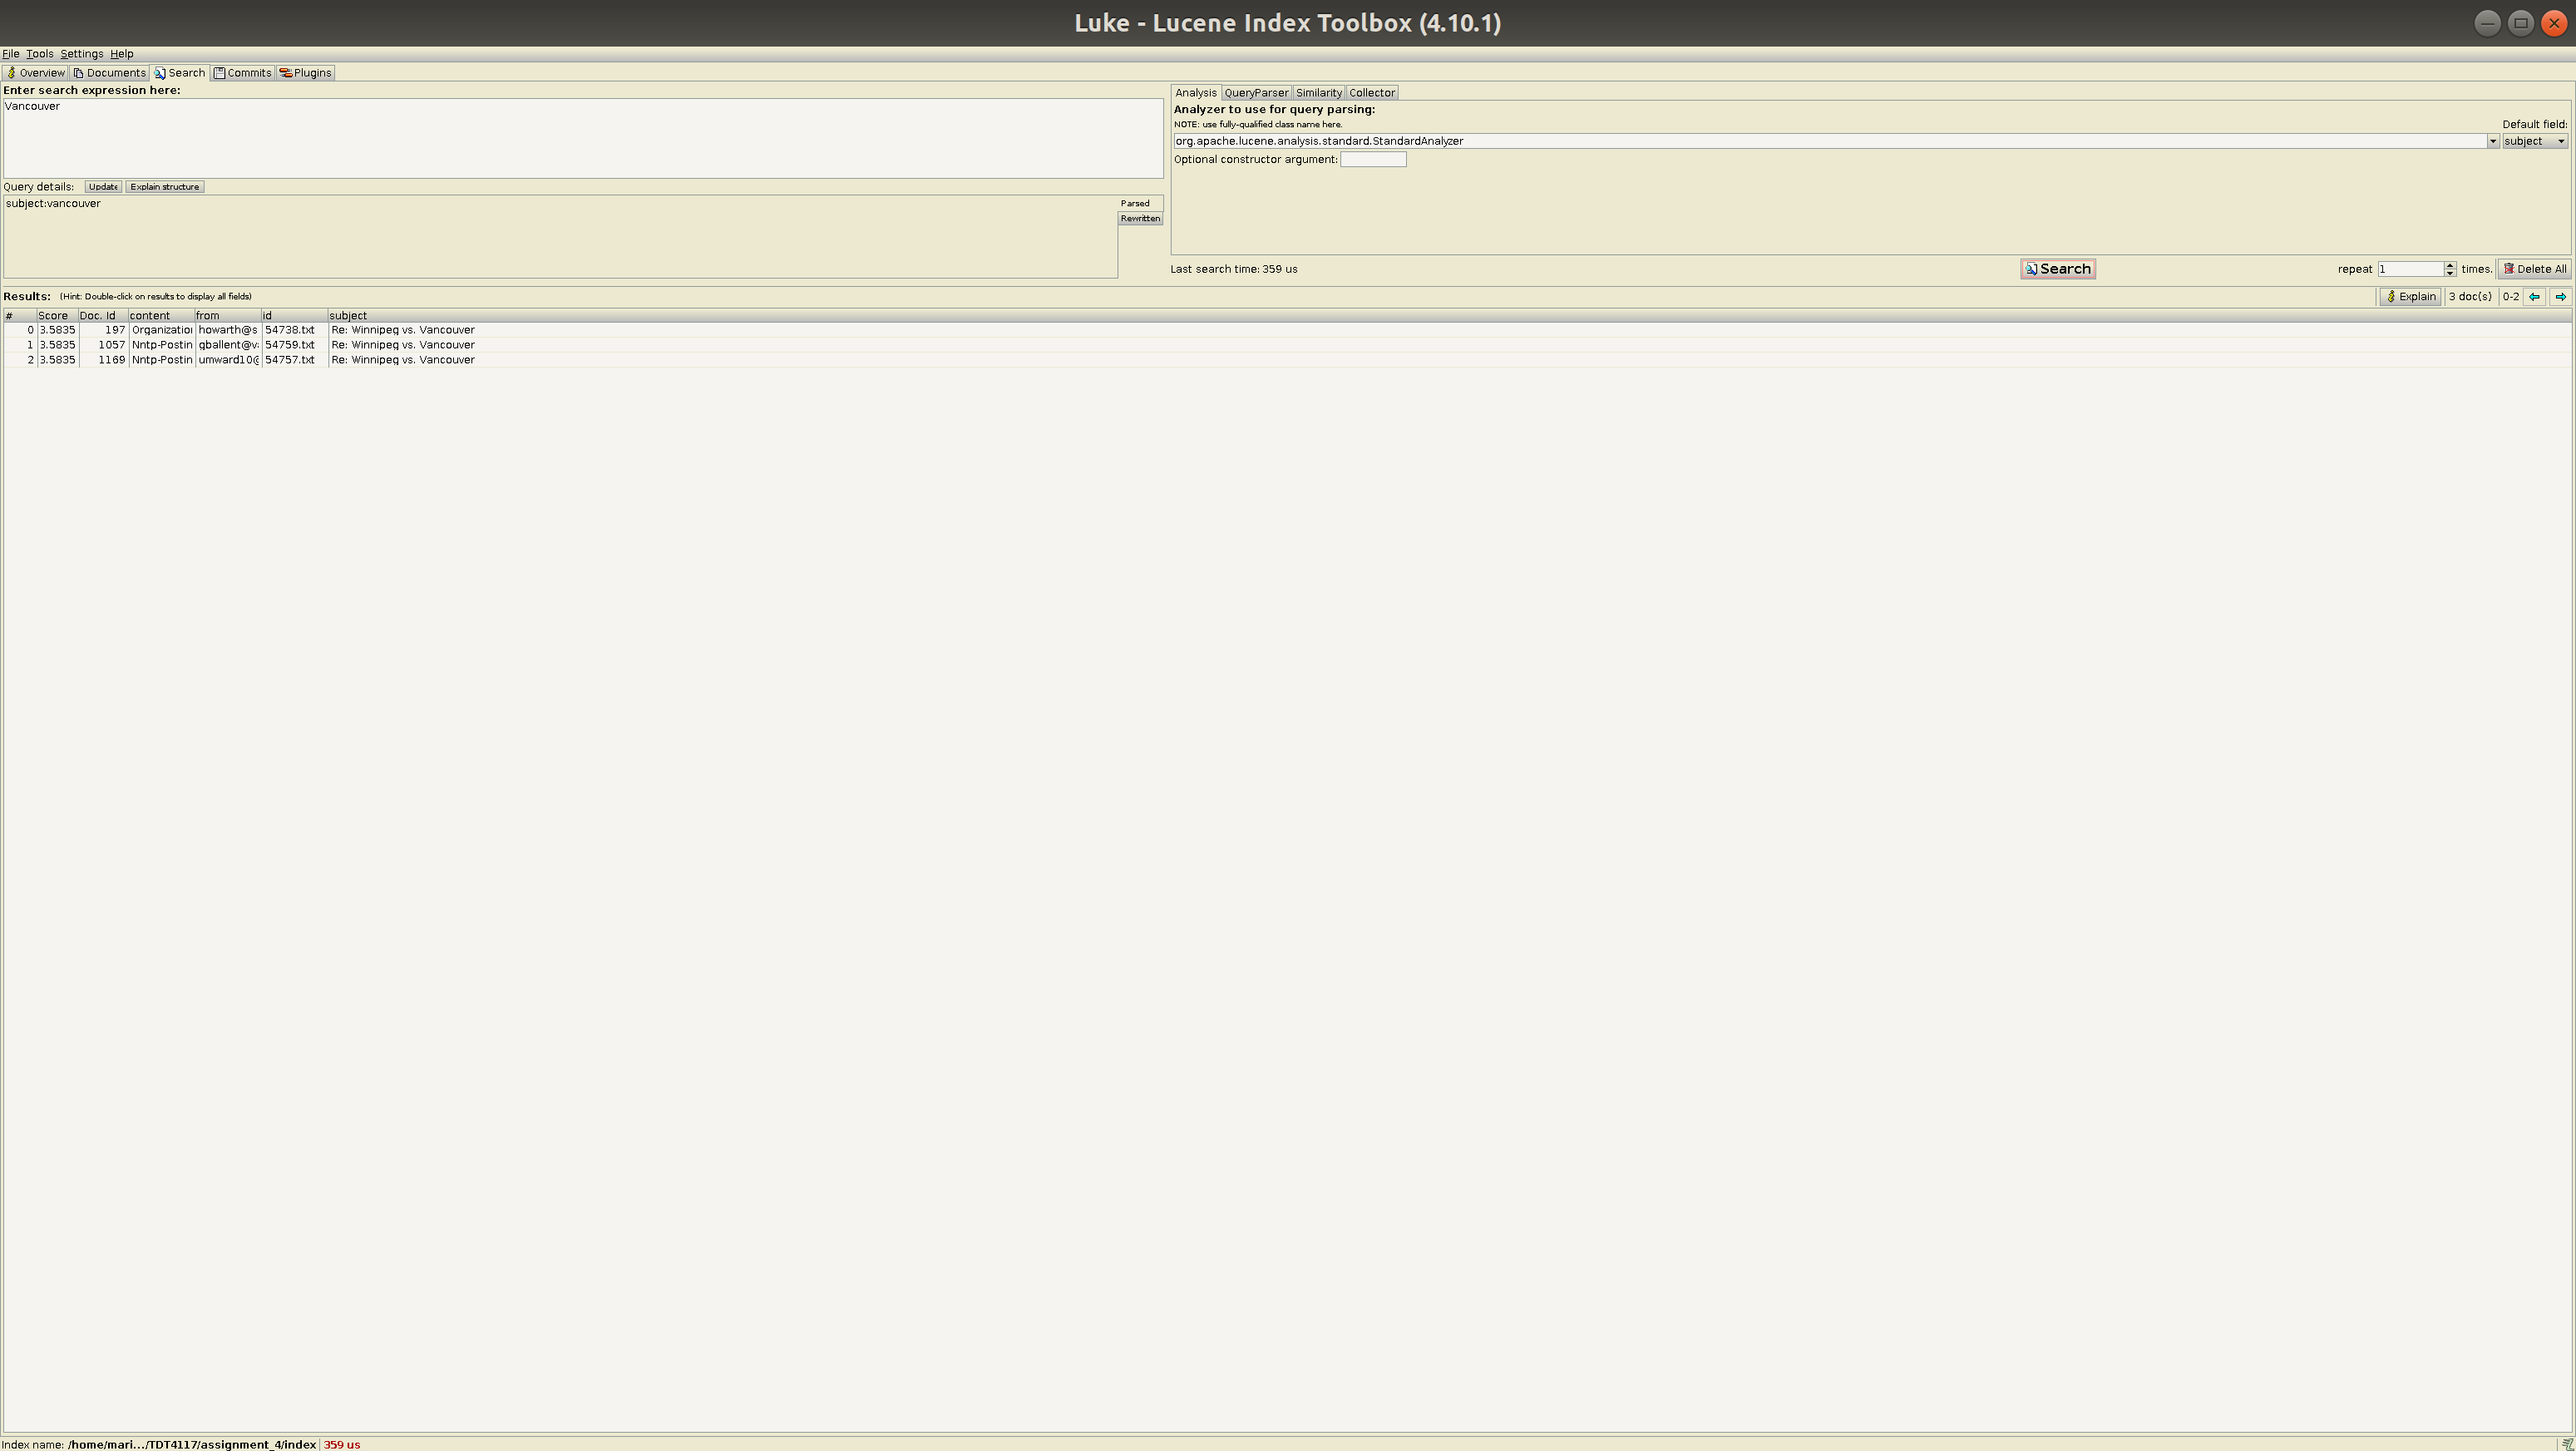
\includegraphics[width=\textwidth]{subject}
    \caption{Searched for Vancouver in subject}
    \label{fig:subject}
\end{figure}
\end{document}
